\chapter{Introduction}
\label{cha:introduction}
% Intro should be readable to a non expert

\section{Goal}

Complex systems are systems composed of many interconnected elements that 
interact with each other, often in non-linear ways, giving rise to emergent 
properties that cannot be explained by the properties of the individual 
elements alone. In many natural complex systems, learning is a key process that 
allows the system to adapt and evolve over time. 
In this thesis, we explore complex systems
as a framework for studying learning and adaptation in natural and artificial
systems. The aim of this thesis is to develop methods for studying and using
computations that take place in complex dynamical systems to eventually create
learning algorithms that require limited to no supervision. 
Complex systems are systems made up of many interacting components that often 
exhibit non-linear and emergent behaviors that cannot be fully understood by 
analyzing the individual parts of the system in isolation. They often exhibit 
features such as self-organization, adaptation, feedback loops, and the capacity
to undergo phase transitions, all of which can make them challenging to model and 
predict. Examples of complex systems that occur naturally include ecosystems, weather patterns, financial 
markets, social networks, and biological organisms.
This objective is broken down into the following subgoals:

\begin{enumerate}
  \item The first subgoal is to identify complex dynamical systems that have the 
  potential to display emergent open-ended growth, which refers to the ability of 
  a system to spontaneously generate new levels of complexity over time without 
  reaching a state of equilibrium. This growth is often associated with 
  evolutionary-like properties, such as variation, selection, and inheritance.
  There are many ways to define complex systems, and as
        illustrated in Figure \ref{fig:comparison_ca}, some may exhibit more
        interesting and promising behaviors than others. A cellular automaton (CA) 
        is an instance of a complex system that can be described as a grid of cells that can 
        take on a finite set of states and change their state over time according to a set 
        of rules that depend on the states of their neighboring cells. Interesting \acp{CA}, such 
        as the one shown in Figure \ref{fig:structured_sys}
        may be hard to find depending on how the
        search space is defined. The work presented in Chapter
        \ref{cha:meas-compl-evolv} aims to construct a metric of complexity
        that can help to identify interestingly behaving complex
        dynamical systems.
\begin{figure}[htbp]
  \centering
\begin{subfigure}[t]{.4\linewidth}
  \centering
  
\includegraphics[width=\linewidth]{figures/disord2.png}
  \caption{A disordered \acl{CA}.}
 \label{fig:disordered_sys}
\end{subfigure}
\hspace{30pt}
\begin{subfigure}[t]{.4\linewidth}
  \centering
  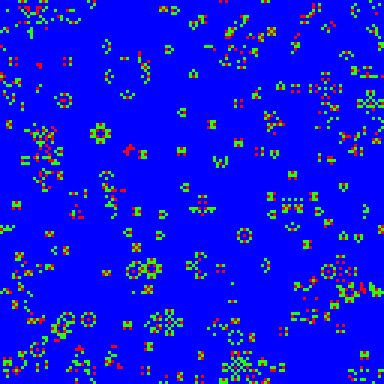
\includegraphics[width=\linewidth]{figures/micro4.png}
  \caption{A \acl{CA} with visible emergent structures.}
  \label{fig:structured_sys}
\end{subfigure}
\caption{Two examples of complex systems (\acf{CA}) with different behavior
  types. \ref{fig:structured_sys} and \ref{fig:disordered_sys} show a single state 
  of a randomly initialized 2D \ac{CA} simulated for a fixed number of steps. Some \acp{CA} 
  appear more promising than others for the design of
  unsupervised learning systems because of their emergent complex structures
  (visible in \ref{fig:structured_sys}), whereas the \ac{CA} in
  \ref{fig:disordered_sys} seems to behave randomly.}
  \label{fig:comparison_ca}
\end{figure}

  \item The second subgoal is to measure the fraction of systems that have the most complex and rapidly
        evolving behavior. Defining these notions is also part of the goal.
        This subgoal is distinct from the first one, which focuses on complex system design in 
        general. Instead, this subgoal involves establishing approaches to evaluate growth 
        in complexity.
        We believe that systems with the most complex and rapidly
        evolving behavior are promising for further use since
        they may exhibit open-ended complexity growth. In Chapters
        \ref{cha:meas-compl-evolv} and \ref{cha:visu-comp-large}, we present
        different methods to measure evolving complexity and understand when the
        complexity increases over time. Chapter \ref{cha:visu-comp-large} of this thesis is dedicated to investigating the importance of multiscale analysis for the complexity of
        cellular automata, which is the process of studying a system at different levels of detail or resolution.   Additionally, we identify complex systems with behavior that
        changes when we manipulate the scale of the system, either by increasing or decreasing its size.
\begin{figure}[htbp]
  \centering
 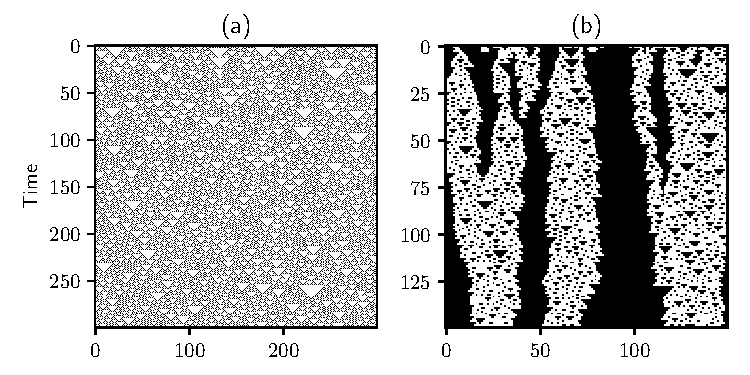
\includegraphics[width=.9\linewidth]{figures/rule18_small}
 \caption{Filtering the behavior of elementary \acl{CA} rule 18. This
   uncovers a highly structured behavior with the propagation of area boundaries
   within the apparent randomness. (a) shows 300 timesteps
of a randomly initialized rule 18 simulation. Notice the complex structures made
visible in (b) with a filtering method. This Figure is discussed in more details in Chapter \ref{cha:visu-comp-large}.}
  \label{fig:rule_18}
\end{figure}

  \item Apply promising systems to challenging learning tasks where classical
        machine learning models may fail or become less efficient. The goal is to
        define various ways to apply evolving complex dynamical systems to some
        standard learning tasks and to find out if it improves the performance
        or efficiency of the learning algorithm. An example application that we
        explore in Chapter \ref{cha:learn-effic-compl} is illustrated in
        Figure~\ref{fig:ca_lm}, where a \ac{CA} is used to implement a language
        model, a probabilistic model that is used to generate text to complete
        sentences. In Chapter \ref{cha:background}, we explore the similarities
        between \acp{CA} networks and highlight the numerous potential applications of \acp{CA}.
\begin{figure}[htbp]
  \centering
  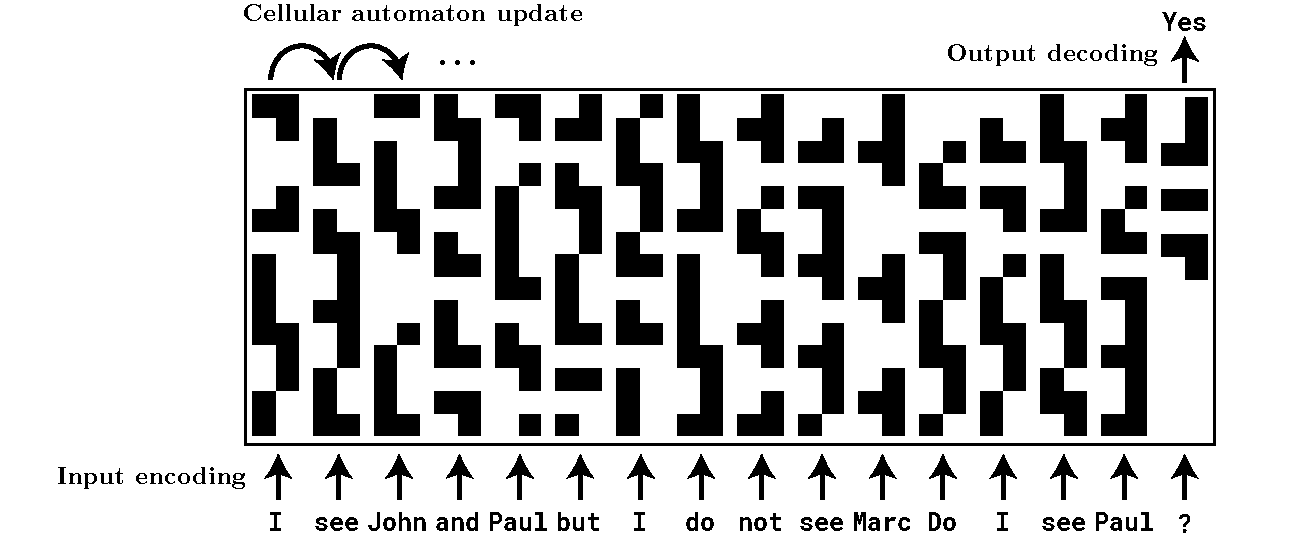
\includegraphics[width=\linewidth]{figures/ca_lm}
  \caption{An example of using a \acl{CA} and reservoir computing to implement a
    language model. Tokens are encoded within the \acl{CA} internal state. The
    \acl{CA} update rule is then applied and an output value is decoded from the
    final state. Each vertical bar represents two consecutive internal \ac{CA} states, which 
    are enriched with the encoded input.}
  \label{fig:ca_lm}
\end{figure}

\end{enumerate}

In this thesis, we do not focus our attention on what the machine learning
community commonly refers to as ``unsupervised learning'', that is, learning
structure from unlabeled data
\parencite{hintonUnsupervisedLearningFoundations1999}. In machine learning,
supervision refers to a label, a number, or a collection of numbers that
represents an expected outcome associated with some input data. Our goal is to
construct models that can develop autonomously without necessarily needing any external data or
interactions. Therefore, we first seek systems that behave that way on their
own and postpone the issue of learning to optimize a particular objective
function to the end of the thesis (Chapter \ref{cha:learn-effic-compl}). 
We are particularly interested in systems that can develop through
internal evolution rules without any input, which is the case for many complex
systems.

Throughout the thesis, we work toward achieving these goals, focusing on one
particular complex system: the \acl{CA} \parencite{vonneumannTheorySelfreproducingAutomata1966}. This model has been extensively studied
due to its simple definition and ability to simulate a wide range of complex
behaviors. We provide a detailed description of cellular automata in Section
\ref{sec:cellular-automata-sec}. This thesis provides new insights into the role
of learning in complex systems and open-ended evolution and demonstrates the
potential of cellular automata as a model for studying these phenomena.

\section{Motivation}\label{sec:motivation}

It is possible that some form of evolutionary mechanism may be necessary in
order to achieve advanced forms of artificial intelligence (AI), particularly 
if the goal is to create
intelligent systems that can adapt and learn in complex and changing
environments. Complex dynamical systems could be key to overcome the problems
with existing learning algorithms, such as difficulties in generalization,
robustness, or the ability to learn continuously
\parencite{parisiContinualLifelongLearning2019}. The natural intelligence of
biological systems seems to depend on emerging properties selected through
evolution. For example, biological life exhibits a pattern of major evolutionary
transitions in which autonomously replicating entities at the lower level merged to form a
single more complex corporate body
\parencite{lorenzEmergenceModularityBiological2011}. This is believed to have
occurred for the emergence of eukaryotic cells, as well as for multicellular
life \parencite{hammerschmidtLifeCyclesFitness2014}. All complex and diverse
biological entities have presumably emerged from a single common ancestor and,
even before, from inorganic components present on the surface of the Earth
\parencite{woeseUniversalAncestor1998, smithOriginsLifeBirth2000}.

So far, it remains uncertain which algorithmic characteristics might enable 
an artificial system to exhibit a path comparable to the natural evolutionary
process within its state space, which involves the transition from basic 
constituents to intricate entities. Producing emerging
phenomena similar to those of nature \emph{in silico} is a long-standing
challenge. There are many algorithms that attempt to mimic evolutionary
properties to solve particular tasks, called evolutionary algorithms
\parencite{fogelArtificialIntelligenceSimulated1966,
  ,millerDesigningNeuralNetworks1989, backOverviewEvolutionaryAlgorithms1993}.
However, many of these methods focus on searching the space of solutions using
high-level evolutionary mechanisms, such as genetic mutations and crossovers.
Although effective in solving precise tasks, these methods often obscure another
crucial component of natural evolution by using an explicit fitness function.

Most existing machine learning algorithms rely on the choice of an objective
function: a clearly defined mapping from the current state and parameters of a
model to a real value, which indicates the performance of that model. The
function depends on the objective of the model. For a supervised learning
problem, we may count the number of misclassified objects or the distance
between the predictions and the expected results. Even in unsupervised learning,
the family of algorithms used for learning from unlabeled data, objectives are
still central. For example, the well-known K-means clustering algorithm minimizes
the sum of square distances to cluster centers.

This reliance on objective functions creates two main issues: (i) the objective
is not always clearly defined or can be too broad for general-purpose
applications. For example, a possible objective function of a walking robot
could be ``not fall when stepping through its surrounding environment''. This
function is impractical to define and will vary greatly depending on the
parameters of the environment (e.g. depending on the terrain, malfunctioning or 
missing limbs of the robots). Indirect rewards such as ``head not touching the ground''
may help, but it does not cover all possible ways the model could fail. 
This problem of defining an objective is still present in our goal of designing
a general-purpose, autonomously developing learning algorithm.
Furthermore, (ii) using predefined functions as goals can be counterproductive
because, as many examples in nature demonstrate, robust paths to complex
objectives are often deceptive. They involve developing in unexpected directions
that may initially seem to be against the original goal
\parencite{stanleyWhyGreatnessCannot2015}.

In this thesis, the term \emph{unsupervised} refers to a form of learning with
no predefined objective. Like in natural evolution, we expect true unsupervised
algorithms to develop new features autonomously and become progressively more
complex over time. Such algorithms would regularly learn to solve problems on
their own without the need to be explicitly guided towards the problem solutions, 
thereby discovering robust
and diverse solutions to deceptive problems.


\section{Challenges}\label{sec:challenges}

\begin{figure}[htbp]
  \centering
  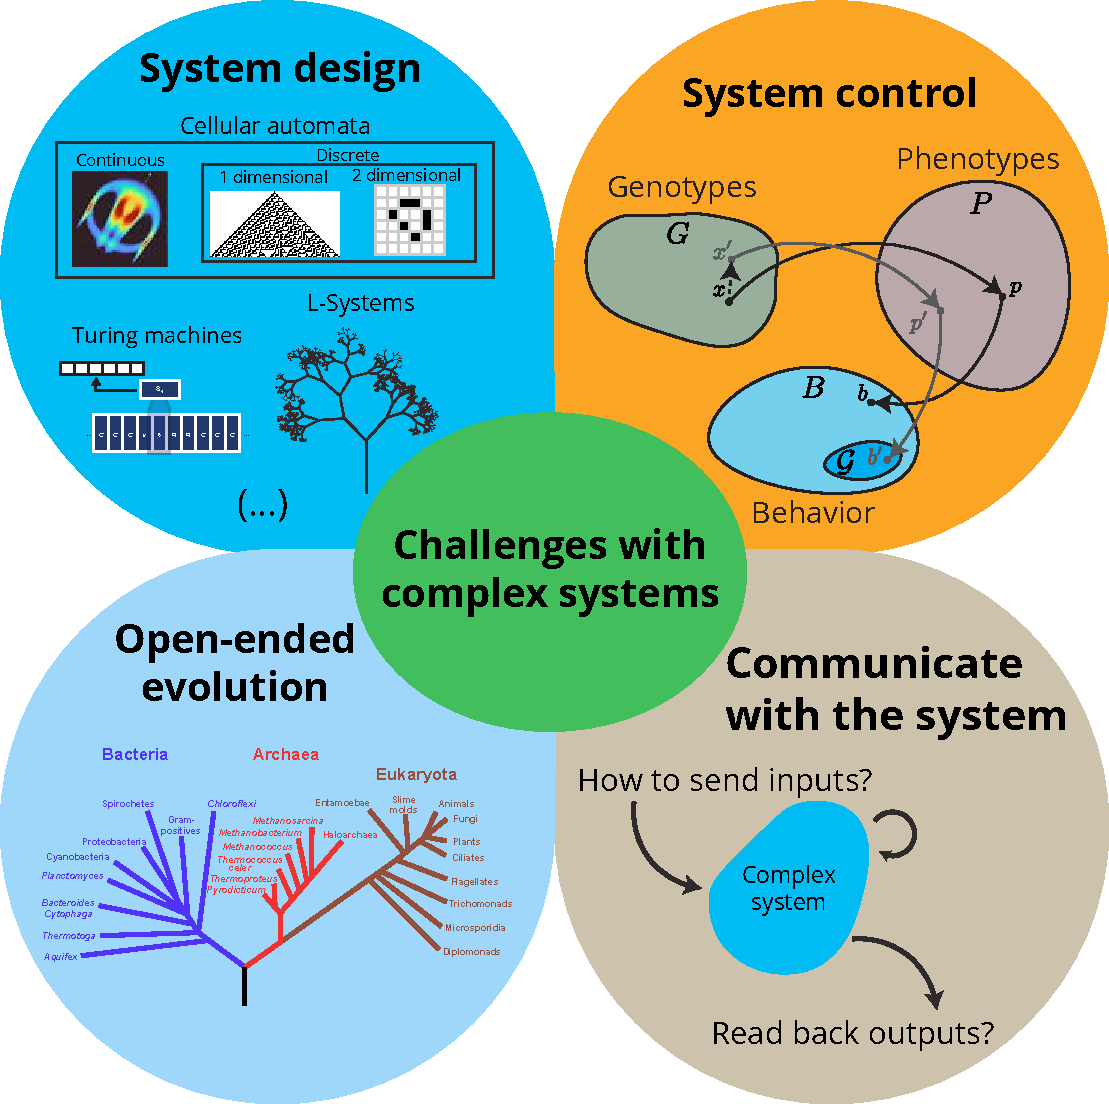
\includegraphics[width=.98\linewidth]{figures/challenges}
  \caption{The challenges of working with complex systems encountered across
    this thesis can be broken down in several categories. \textbf{(1)} The choice
    and design of the system, \textbf{(2)} the control of the system which
    involves understanding the complex mapping between a parameter space and the
    possibly unpredictable behavior of a system, \textbf{(3)} the search for
    open-ended evolution properties similar to the ones found in nature,
    \textbf{(4)} the issue of sending inputs and reading outputs from the
    internal state of a complex system. This illustration uses
    \href{https://commons.wikimedia.org/wiki/File:Lenia_icon4.png}{Lenia
      icon4.png} by Bert Wang-Chak Chan, licensed under
    \href{https://creativecommons.org/licenses/by-sa/4.0/}{CC BY 4.0}. }
  \label{fig:challenges}
\end{figure}

The study of complex systems presents a range of difficult challenges by itself
\parencite{sanmiguelChallengesComplexSystems2012}. 
The complexity of a system is an emergent property that arises from various factors, 
including its intricate structure, the number of elements it contains, how it functions, 
and how it responds to different kinds of external influences. These factors contribute 
to the overall complexity of the system, which could be measured in various ways.
For many complex systems, their emergent mechanisms are
poorly understood. We identify four main challenges associated with the study of
complex systems: (i) the questions of the design choices in defining and sampling a
complex system (section \ref{sec:design-compl-syst}), (ii) which will in turn define
their potential to support a form of open-ended evolution (section
\ref{sec:open-ended-evolution}) and (iii) how we can expect to build an interface to
communicate with it (section \ref{sec:compl-syst-inputs}), (iv) which is essential to
achieve some form of control of that system (section \ref{sec:compl-syst-contr}).

\subsection{Design of a complex system\label{sec:design-compl-syst}}

The first challenge is to construct a suitable complex system. The definition of a 
complex system is broad, and several systems with
interesting dynamics have been studied under that name. For example, abstract models such as L-Systems (formal grammars used to model the growth and development of organic structures),
Random Boolean networks (dynamical systems that consist of a fixed number of binary nodes 
that are randomly connected to each other and updated based on the state of its neighboring 
nodes), Turing machines (abstract deterministic computing machines consisting of a tape and 
a read-write head), and \Acfp{CA}. In this thesis, we
focus mainly on the last listed element: the \acl{CA}. There are multiple
benefits to working with this model. It is very simple to define, and its high
parallelism makes its implementation straightforward. Moreover, \acp{CA} have
shown the ability to simulate a wide range of complex behaviors
\parencite{wolframNewKindScience2002}.

Choosing the right complex system architecture is essential because it defines
the search space over which interesting and useful systems can be found.
Correctly parameterizing that space can also be challenging because too many
degrees of freedom make it difficult to search for and find good systems, while
too few might indicate a lack of expressivity. An example parameterization of
\ac{CA} with little expressivity is Langton's lambda parameter
\parencite{langtonComputationEdgeChaos1990}. At the other end of the spectrum, the
\ac{CA} rule is a simple parametrization with many degrees of freedom, which
makes it impractical.

Even when we limit ourselves to the study of \ac{CA}, many variants can be
considered. Cellular automata can have continuous or discrete states and operate
in continuous or discrete space. For discrete state and space cellular automata,
the number of states and the window of the update function can vary, as well as the
topology of the simulation space. We tackle this issue from various angles
across the thesis, exploring the question of rule definition in Chapter
\ref{cha:meas-compl-evolv}, the scale in Chapter \ref{cha:visu-comp-large} and
the connectivity pattern in Chapter \ref{cha:learn-effic-compl}.

\subsection{Complex systems control}\label{sec:compl-syst-contr}

\begin{figure}[htbp]
  \centering
  \begin{subfigure}[t]{.47\linewidth}
    \centering
    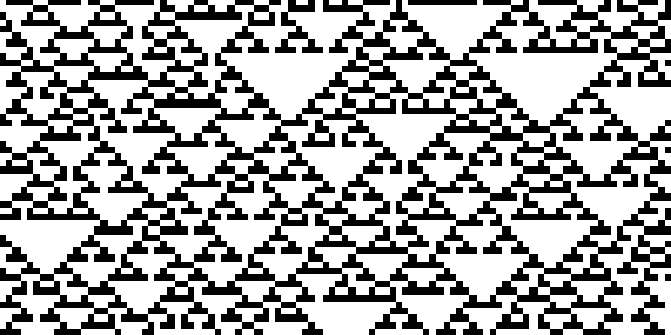
\includegraphics[width=.93\linewidth]{figures/ca_comp_a}
    \caption{\ac{CA} rule 22 on a tape of size 100, ran for 50 steps from a
      random initial state.}
    \label{fig:ca_comp_a}
  \end{subfigure}
  \hspace{10pt}
  \begin{subfigure}[t]{.47\linewidth}
    \centering
    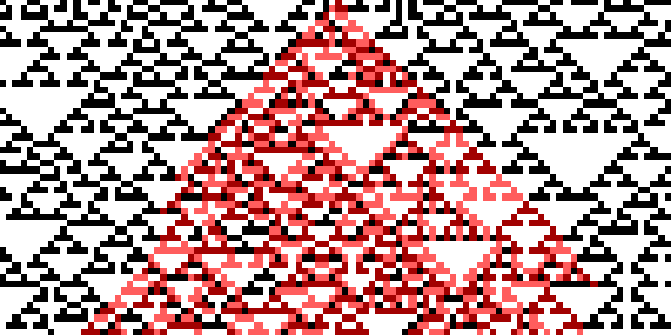
\includegraphics[width=.93\linewidth]{figures/ca_comp_b}
    \caption{\ac{CA} rule 22 on a tape of size 100, ran from a slightly
      different initial state. The cells different from Figure \ref{fig:ca_comp_a} are
      overlayed in red.}
    \label{fig:ca_comp_b}
  \end{subfigure}

  \caption{Comparison of the same 1 dimensional \ac{CA} ran from two initial conditions
    differing only by one cell. Each row is the state of the \ac{CA} at one time
    step, with time increasing from top to bottom. The effect of the small perturbation 
    of initial conditions grows rapidly as the \ac{CA} evolves in time.}
  \label{fig:ca_comp}
\end{figure}


Even if we want complex systems that evolve in unexpected directions and grow in
an open-ended way without supervision, it may still be useful to steer them
locally towards specific targets. A major challenge that follows from this goal
is that many complex systems are chaotic. Deterministic dynamical systems can 
exhibit behavior that is extremely sensitive to their initial conditions. This sensitivity 
is sometimes referred to as chaos, where even tiny perturbations in the initial conditions 
can result in significantly different outcomes or trajectories. This is illustrated 
with a simple \ac{CA} rule in Figure \ref{fig:ca_comp}. 
Because of this property, it is often very hard to predict how a
given system will evolve over time, and therefore hard to steer its evolution
towards a particular final state or along a chosen trajectory. While it can be challenging 
to apply these systems to certain basic tasks, their ability to generate unexpected solutions 
to difficult problems is an advantage in developing open-ended systems. Such systems 
need to continually produce new and diverse solutions, without a 
predefined endpoint, and the sensitivity to initial conditions an advantage in 
achieving this goal.

This problem is also related to the issue of sending a control signal to a
complex system that depends on the choice of encoding for that signal. This
encoding can significantly impact the system's ability to respond to the control 
signal and generate the desired outcome. 

\subsection{Complex systems inputs and outputs\label{sec:compl-syst-inputs}}

Some of the complex systems we study in this thesis are closed systems. They do
not expect inputs or have any well-defined outputs. For example, \ac{CA} and
\ac{RBN} do not have a notion of inputs and outputs built into the model. They
are standalone objects that evolve according to a set of internal rules.

A common challenge for such systems is to define the inputs and outputs in a way
that preserves their internal dynamics. This is also connected to the control
problem of Section \ref{sec:compl-syst-contr}, because controlling a complex
system implies being able to send a control signal and read the current
state of the system.

Throughout this work, we use a framework called \emph{reservoir computing} (RC) for this 
purpose. Reservoir
computing allows one to harvest the internal computations of complex systems, or
\emph{read} information from its internal state by learning a linear regression
that maps that internal state to desired outputs (see Section
\ref{sec:res-models}).



\subsection{Open-ended evolution without
  objectives}\label{sec:open-ended-evolution}

Another challenge is posed by the lack of a clear objective in the design of
unsupervised learning systems. Even without an objective, it is still essential
to understand which complex systems to choose from all available options or how
to tune their parameters so that they behave in interesting ways. For example,
\acp{CA} such as the one shown in Figure \ref{fig:disordered_sys} are unlikely 
to be useful for constructing systems that demonstrate a growth of complexity 
due to their disordered nature in both space and time. As a result, they cannot
preserve information about the past.

Because our goal is to create a system that has the property of evolving in an
open-ended way, we need metrics that can help select systems. However, these metrics 
should not be used as an additional objective function, as doing so would result 
in the problems described in Section \ref{sec:motivation}. We address this 
challenge in particular
in Chapter~\ref{cha:meas-compl-evolv}, by designing a complexity metric that can
help select interesting complex systems, without relying on a specific
task-based performance score.

\section{Contributions}

The main contributions of this thesis are as follows.
\begin{enumerate}
  \item Our first contribution is a review of the literature (Chapter \ref{cha:literature-review})
        describing the connections between cellular automata
        and other complex systems, open-ended evolution, and neural networks.
        Studying these fields from a single point of view is a relatively novel
        endeavor, and we consider a review necessary to place the rest of our
        work in its context.

  \item Our second contribution is the development of a general complexity metric that can help identify
        complex systems with interesting behavior (Chapter \ref{cha:meas-compl-evolv}). Our findings were published in \cite{cisnerosEvolvingStructuresComplex2019}.

  \item The third contribution is the development of a coarse-graining method to visualize computations in
        cellular automata and other discrete systems with local interactions (Chapter \ref{cha:visu-comp-large}). Our findings were published in \cite{cisnerosVisualizingComputationLargescale2020}.

  \item Our fourth contribution is the introduction of a metric for learning efficiency for learning
        algorithms as well as a benchmark dataset of progressively harder
        language tasks (Chapter \ref{cha:learn-effic-compl}). Our findings were published in \cite{cisnerosBenchmarkingLearningEfficiency2022}.
\end{enumerate}

\section{Thesis overview}


Chapter \ref{cha:background} presents some background notions about complex
systems, cellular automata, and reservoir computing.

In Chapter \ref{cha:literature-review}, we review relevant methods and tools for
measuring the complexity of complex systems and using their computations for
various tasks.

Chapter \ref{cha:meas-compl-evolv} introduces a complexity metric that allows us 
to select complex systems with interesting behavior. The metric measures the
``novelty'' of the temporal states of a system compared to a reference one. We
built a dataset of interesting cellular automata to validate the quality of the
metric.

Chapter \ref{cha:visu-comp-large} addresses the question of large-scale complex
systems and the applicability of complexity metrics at multiple scales. We
propose three algorithms for the coarse-graining of cellular automata. This allows
us to reduce the size of large-scale systems while retaining the interesting parts
of the behavior.

Chapter \ref{cha:learn-effic-compl} presents a learning efficiency metric and a
dataset to measure the speed of learning of various systems. We show that
reservoir computing-based systems using cellular automata can be more efficient
than usual machine learning algorithms in constrained data and computation
settings.

Chapter \ref{cha:future_work} outlines potential avenues for further research in 
the field. It provides suggestions for how the current work could be expanded or 
improved, highlighting areas that require additional investigation to advance the 
understanding of the subject. We propose some experiments that could extend the 
potential applications of cellular automata, as well as a theoretical framework 
for learning in dynamical systems.

Finally, Chapter \ref{cha:conclusion} summarizes our contributions in this thesis. 

\section{Publications and software}

The thesis has led to the following publications.

\begin{itemize}
  \item \fullcite{cisnerosEvolvingStructuresComplex2019}
  \item \fullcite{cisnerosVisualizingComputationLargescale2020}
  \item \fullcite{cisnerosBenchmarkingLearningEfficiency2022}
\end{itemize}

The code to reproduce the experiments of all three publications is available on
GitHub: \url{https://github.com/hugcis/evolving-structures-in-complex-systems},
\url{https://github.com/hugcis/benchmark_learning_efficiency}. We also published a
dataset that we used for our benchmark in our last
publication. It is available at
\url{https://github.com/hugcis/incremental_tasks/}.
